\documentclass[12pt]{article}
\usepackage[paper=letterpaper,margin=1.5cm]{geometry}
\usepackage{amsmath}
\usepackage{amssymb}
\usepackage{amsfonts}
\usepackage{mathtools}
%\usepackage[utf8]{inputenc}
%\usepackage{newtxtext, newtxmath}
\usepackage{lmodern}     % set math font to Latin modern math
\usepackage[T1]{fontenc}
\renewcommand\rmdefault{ptm}
%\usepackage{enumitem}
\usepackage[shortlabels]{enumitem}
\usepackage{titling}
\usepackage{graphicx}
\usepackage[colorlinks=true]{hyperref}
\usepackage{setspace}
\usepackage{subfigure} 
\usepackage{braket}
\usepackage{color}
\usepackage{tabularx}
\usepackage[table]{xcolor}
\usepackage{listings}
\usepackage{mathrsfs}
\usepackage{stackengine}
\usepackage{physics}
\usepackage{afterpage}
\usepackage{pdfpages}
\usepackage[export]{adjustbox}
\usepackage{biblatex}

\setstackEOL{\\}

\definecolor{dkgreen}{rgb}{0,0.6,0}
\definecolor{gray}{rgb}{0.5,0.5,0.5}
\definecolor{mauve}{rgb}{0.58,0,0.82}


\lstset{frame=tb,
  language=Python,
  aboveskip=3mm,
  belowskip=3mm,
  showstringspaces=false,
  columns=flexible,
  basicstyle={\small\ttfamily},
  numbers=none,
  numberstyle=\tiny\color{gray},
  keywordstyle=\color{blue},
  commentstyle=\color{dkgreen},
  stringstyle=\color{mauve},
  breaklines=true,
  breakatwhitespace=true,
  tabsize=3
}
\setlength{\droptitle}{-6em}

\makeatletter
% we use \prefix@<level> only if it is defined
\renewcommand{\@seccntformat}[1]{%
  \ifcsname prefix@#1\endcsname
    \csname prefix@#1\endcsname
  \else
    \csname the#1\endcsname\quad
  \fi}
% define \prefix@section
\newcommand\prefix@section{}
\newcommand{\prefix@subsection}{}
\newcommand{\prefix@subsubsection}{}
\renewcommand{\thesubsection}{\arabic{subsection}}
\makeatother
\DeclareMathOperator*{\argmin}{argmin}
\newcommand{\partbreak}{\begin{center}\rule{17.5cm}{2pt}\end{center}}
\newcommand{\alignbreak}{\begin{center}\rule{15cm}{1pt}\end{center}}
\newcommand{\tightalignbreak}{\vspace{-5mm}\alignbreak\vspace{-5mm}}
\newcommand{\hop}{\vspace{1mm}}
\newcommand{\jump}{\vspace{5mm}}
\newcommand{\R}{\mathbb{R}}
\newcommand{\C}{\mathbb{C}}
\newcommand{\N}{\mathbb{N}}
\newcommand{\G}{\mathbb{G}}
\renewcommand{\S}{\mathbb{S}}
\newcommand{\bt}{\textbf}
\newcommand{\xdot}{\dot{x}}
\renewcommand{\star}{^{*}}
\newcommand{\ydot}{\dot{y}}
\newcommand{\lm}{\mathrm{\lambda}}
\renewcommand{\th}{\theta}
\newcommand{\id}{\mathbb{I}}
\newcommand{\si}{\Sigma}
\newcommand{\Si}{\si}
\newcommand{\inv}{^{-1}}
\newcommand{\T}{^\intercal}
\renewcommand{\tr}{\text{tr}}
\newcommand{\ep}{\varepsilon}
\newcommand{\ph}{\varphi}
%\renewcomand{\norm}[1]{\left\lVert#1\right\rVert}
\definecolor{cit}{rgb}{0.05,0.2,0.45}
\addtolength{\jot}{1em}
\newcommand{\solution}[1]{

\noindent{\color{cit}\textbf{Solution:} #1}}

\newcounter{tmpctr}
\newcommand\fancyRoman[1]{%
  \setcounter{tmpctr}{#1}%
  \setbox0=\hbox{\kern0.3pt\textsf{\Roman{tmpctr}}}%
  \setstackgap{S}{-.9pt}%
  \Shortstack{\rule{\dimexpr\wd0+.1ex}{.9pt}\\\copy0\\
              \rule{\dimexpr\wd0+.1ex}{.9pt}}%
}

\newcommand{\Id}{\fancyRoman{2}}

% Enter the specific assignment number and topic of that assignment below, and replace "Your Name" with your actual name.
\title{STAT 37710: Homework 1}
\author{Caleb Derrickson}
\date{March 29, 2024}

\begin{document}
\onehalfspacing
\maketitle
\allowdisplaybreaks
{\color{cit}\vspace{2mm}\noindent\textbf{Collaborators:}} The TA's of the class, as well as Kevin Hefner, and Alexander Cram.

\tableofcontents

\newpage
\section{Problem 1}
As we saw in class, $k$-means clustering minimizes the average square distance distortion
\begin{align}
    J_{avg^2} = \sum_{j = 1}^k\sum_{\textbf{x} \in C_j} d(\textbf{x}, \textbf{m}_j)^2, \label{Javg}
\end{align}
where $d(\textbf{x}, \textbf{x}') = \norm{\textbf{x} - \textbf{x}'}$ and $C_j$ is the set of points belonging to cluster $j$. Another distortion function that we mentioned is the intra-cluster sum of squared distances,
\[J_{IC} = \sum_{j = 1}^k \frac{1}{|C_j|}\sum_{\textbf{x} \in C_j} \sum_{\textbf{x}' \in C_j} d(\textbf{x}, \textbf{x}')^2.\]

\partbreak
\subsection{Problem 1, part a}
Given that in $k$-means, $\textbf{m}_j = \frac{1}{|C_j|}\sum_{\textbf{x} \in C_j} \textbf{x}$, show that $J_{IC} = 2J_{avg^2}$.
\partbreak
\begin{solution}

    Fix $j \in \{1, 2, ..., k\}$, that is, let us focus on one cluster. The two distortion functions for cluster $j$ would then be 
    \[J_{avg^2} = \sum_{\textbf{x} \in C_j}d(\textbf{x}, \textbf{m}_j)^2, \quad J_{IC} = \frac{1}{|C_j|} \sum_{\textbf{x} \in C_j}\sum_{\textbf{x}' \in C_j} d(\textbf{x}, \textbf{x}')^2.\]

    Starting with the intra-cluster distortion, we will show the equality for $C_j$.

    \tightalignbreak
    \begin{align*}
        &J_{IC} = \frac{1}{|C_j|} \sum_{\textbf{x} \in C_j}\sum_{\textbf{x}' \in C_j} d(\textbf{x}, \textbf{x}')^2 &\text{(Given.)}\\
        &= \frac{1}{|C_j|} \sum_{\textbf{x} \in C_j}\sum_{\textbf{x}' \in C_j} (\textbf{x} - \textbf{x}')\T (\textbf{x} - \textbf{x}') &\text{(Euclidean distance.)}\\
        &= \frac{1}{|C_j|} \sum_{\textbf{x} \in C_j}\sum_{\textbf{x}' \in C_j} \left[ \textbf{x}\T \textbf{x} - 2\textbf{x}\T \textbf{x}' + (\textbf{x}')\T (\textbf{x}')\right] &\text{(Expanding.)}\\
        &= \frac{1}{|C_j|} \sum_{\textbf{x} \in C_j}\sum_{\textbf{x}' \in C_j} \textbf{x}\T \textbf{x} - \frac{2}{|C_j|} \sum_{\textbf{x} \in C_j}\sum_{\textbf{x}' \in C_j}\textbf{x}\T \textbf{x}' + \frac{1}{|C_j|} \sum_{\textbf{x} \in C_j}\sum_{\textbf{x}' \in C_j} (\textbf{x}')\T (\textbf{x}') &\text{(Expanding.)}\\
        &= \sum_{\textbf{x} \in C_j} \textbf{x}\T \textbf{x} - \frac{2}{|C_j|} \sum_{\textbf{x} \in C_j}\sum_{\textbf{x}' \in C_j} \textbf{x}\T \textbf{x}' + \sum_{\textbf{x}' \in C_j} (\textbf{x}')\T (\textbf{x}') &\text{(Independent summations.)}\\ 
        &= \sum_{\textbf{x} \in C_j} \textbf{x}\T \textbf{x} - \frac{2}{|C_j|} \sum_{\textbf{x} \in C_j}\sum_{\textbf{x}' \in C_j} \textbf{x}\T \textbf{x}' + \sum_{\textbf{x}' \in C_j} \textbf{x}\T \textbf{x} &\text{(Dummy index.)}\\
        &= 2\sum_{\textbf{x} \in C_j} \textbf{x}\T \textbf{x} - \frac{2}{|C_j|} \sum_{\textbf{x} \in C_j}\sum_{\textbf{x}' \in C_j} \textbf{x}\T \textbf{x}' &\text{(Simplifying.)}\\
        &= 2\sum_{\textbf{x} \in C_j} \textbf{x}\T \textbf{x} - \frac{4}{|C_j|} \sum_{\textbf{x} \in C_j}\sum_{\textbf{x}' \in C_j} \textbf{x}\T \textbf{x}' + \frac{2}{|C_j|} \sum_{\textbf{x} \in C_j}\sum_{\textbf{x}' \in C_j} \textbf{x}\T \textbf{x}' &\text{(Adding a zero.)}\\
        &= 2\sum_{\textbf{x} \in C_j}\left[ \textbf{x}\T \textbf{x} - \frac{2}{|C_j|} \sum_{\textbf{x}' \in C_j} \textbf{x}\T \textbf{x}' + \frac{1}{|C_j|} \sum_{\textbf{x}' \in C_j} \textbf{x}\T \textbf{x}'\right] &\text{(Grouping Summations.)}\\
        &= 2\sum_{\textbf{x} \in C_j}\left[ \textbf{x}\T \textbf{x} - \frac{2}{|C_j|} \sum_{\textbf{x}' \in C_j} \textbf{x}\T \textbf{x}' + \frac{1}{|C_j|^2} \sum_{\textbf{x}' \in C_j} \sum_{\textbf{x}'' \in C_j} (\textbf{x}')\T \textbf{x}''\right] &\text{(Multiplying by 1.)}\\
        &= 2\sum_{\textbf{x} \in C_j}\left[ \textbf{x}\T \textbf{x} - 2 \textbf{x}\T \left(\sum_{\textbf{x}' \in C_j}\frac{1}{|C_j|}\textbf{x}'\right) + \frac{1}{|C_j|^2} \left(\sum_{\textbf{x}' \in C_j}\textbf{x}'\right)\T \left(\sum_{\textbf{x}'' \in C_j}  \textbf{x}''\right)\right] &\text{(Linearity of inner product.)}\\
        &= 2\sum_{\textbf{x} \in C_j}\left[ \textbf{x}\T \textbf{x} - 2 \textbf{x}\T \textbf{m}_j + \textbf{m}_j \T \textbf{m}_j\right] &\text{(Given form of $\textbf{m}_j$.)}\\
        &= 2\sum_{\textbf{x} \in C_j}\left[ (\textbf{x} - \textbf{m}_j)\T (\textbf{x} - \textbf{m}_j)\right] &\text{(Factoring.)}\\
        &= 2\sum_{\textbf{x} \in C_j} \norm{\textbf{x} - \textbf{m}_j}^2 &\text{(Euclidean Distance.)}\\
        &= 2\sum_{\textbf{x} \in C_j} d(\textbf{x}, \textbf{m}_j)^2 &\text{(Given distance.)}\\
        \implies& J_{IC} = 2J_{avg^2} &\text{(Given.)}
    \end{align*}
    \vspace{-12mm}\alignbreak
    Note that the above proof has only in mind one cluster. It is easy to see however, that this behavior should hold for all clusters since clusters should not overlap (i.e., no point should be assigned to two clusters). Therefore, the claim has been shown. 
\end{solution}

\newpage
\subsection{Problem 1, part b}
Let $\gamma_i \in \{1, 2, ..., k\}$ be the cluster that the $i$-th data-point is assigned to, and assume that there are $n$ points in total, $\textbf{x}_1, \textbf{x}_2, ..., \textbf{x}_n$. Then (\ref{Javg}) can be written as 
\begin{align}
    J_{avg^2}(\gamma_1, ..., \gamma_n, \textbf{m}_1, ..., \textbf{m}_k) = \sum_{i = 1}^n d(\textbf{x}_i, \textbf{m}_{\gamma_i})^2.\label{mod javg}
\end{align}
Recall the $k$-means clustering alternates the following two steps:
\begin{enumerate}
    \item Update the cluster assignments:
    \[\gamma_i \leftarrow \argmin_{j \in \{1, 2, ..., k\}} d(\textbf{x}_i, \textbf{m}_j), \quad i = 1, 2, ..., n.\]
    \item Update the centroids:
    \[\textbf{m}_j \leftarrow \frac{1}{|C_j|} \sum_{i : \gamma_i = j} \textbf{x}_i, \quad j = 1, 2, ..., k. \]
\end{enumerate}
Show that the first of these steps minimizes (\ref{mod javg}) as a function of $\gamma_1, ..., \gamma_n$, while holding $\textbf{m}_1, ..., \textbf{m}_k$ constant, while the second step minimizes it as a function of $\textbf{m}_1, ..., \textbf{m}_k$, while holding $\gamma_1, ..., \gamma_n$ constant. The notation $`` i : \gamma_i = j"$ should be read as ``all $i$ for which $\gamma_i = j"$. 
\partbreak
\begin{solution}

    For the first step, we are given that the updated $\gamma_i$ is chosen such that each point is matched with the closest centroid, for all $i$. Since both the problem of $d(\cdot)$ and $d(\cdot)^2$ are minimized for the same values, we can say that $\gamma_i$ also minimizes the \textit{squared} distances between all points and the centroids. Thus, for the updated $\gamma$, the value of the summation of the squared distances is minimized. Then,
    \[\gamma = \argmin_\gamma \sum_{i = 1}^n d(\textbf{x}_i, \textbf{m}_{\gamma_j})^2 = \argmin_\gamma J_{avg^2}(\gamma, \Vec{\textbf{m}}).\]
    Thus, $\gamma$ minimizes (\ref{mod javg}), while holding the centroids constant. We will now investigate the second update schema. This minimization will be proven in a comparatively methodical manner, taking the gradient of $J_{avg}^2$ and setting it to zero. The gradient with respect to $\textbf{m}$ is then
    \[\grad_\textbf{m} \sum_{i = 1}^n d(\textbf{x}_i, \textbf{m}_{\gamma_j})^2 = -2\sum_{\textbf{x}_i \in C_j} (\textbf{x}_i - \textbf{m}_{\gamma_j})\]
    \newpage
    Setting this equal to zero gives
    \[\sum_{\textbf{x} \in C_j} \textbf{x} = \sum_{\textbf{x}\in C_j} \textbf{m}_{\gamma_j} =|C_j|\textbf{m}_{\gamma_j} \iff \textbf{m}_{\gamma_j} = \frac{1}{|C_j|}\sum_{\textbf{x} \in C_j} \textbf{x}.\]
    Which is what we wanted to find.
\end{solution}

\newpage
\subsection{Problem 1, part c}
Prove that as $k$-means progresses, the distortion decreases monotonically iteration-by-iteration. 
\partbreak
\begin{solution}

    It is easy to see that taking the minimum in each parameter separately will allow the function to iteratively proceed to the minimum. Since each subpart of the $k$-means algorithm minimizes their respective piece, we see that their joined influence produces a lower value than the previous iteration. Therefore, the change in each iteration of $k$-means will provide us a distortion value bounded above by the previous iteration value, implying the algorithm decreases monotonically. 
\end{solution}

\newpage
\subsection{Problem 1, part d}
Give an upper bound on the maximum number of iterations required for full convergence of the algorithm, i.e., the point where neither the centroids, nor the cluster assignments change anymore (note: we do not expect you to prove the bound in Inaba et al., something much looser and simpler will do. 
\partbreak
\begin{solution}

    Note that the elements of $\gamma$ are sampled entirely from the values $\{1, 2, ..., k\}$. If no progress have been made in a new iteration, we surely cannot expect the next iteration to improve as well. This will repeat ad infinitum. Thus, our stopping criterion to ensure no excessive looping is when we observe no (meaningful) change in our chosen distortion function. Initially, $\gamma$ will have a random value, in which each entry is chosen at random. By the previous part, since the algorithm should monotonically decrease our distortion function, no value of $\gamma$ should repeat. In the worst case, the assignment of $\gamma$ will never repeat, only stopping once we have exhausted possible unique values of $\gamma$. Thus, we will see in the worst case our algorithm will iterate $k^n$ times, as we sample values up to $k$, $n$ times. Thus, the iteration is bounded by $k^n$. 
\end{solution}

\newpage
\section{Problem 2}
Implement the $k$-means algorithm in a language of your choice (Python is recommended), initializing the cluster centers randomly, as explained in the slides. The algorithm should terminate when the cluster assignments (and hence, the centroids) don’t change anymore.

\subsection{Problem 2, part a}
The toy dataset \textbf{toydata.txt} contains 500 points in $\R^2$ coming from 3 well separated clusters. Test your code on this data and plot the final result as a 2D plot in which each point’s color or symbol indicates its cluster assignment. Note that because of the random initialization, different runs may produce different results, and in some cases the algorithm might not correctly identify the three clusters. Plot the value of the distortion function as a function of iteration number for 20 separate runs of the algorithm on the same plot. Comment on the plot.
\partbreak
\begin{solution}

    I have implemented the $k$-means algorithm in C++ (just for the experience), and plotted in Python. I will provide the two given plots below. The first plot, Figure \ref{fig:kmeans}, is a scenario where the algorithm reached a global minima: all clusters are being utilized. I make this distinction here, since in Figure \ref{fig:Differentvals}, we see two different convergent values - one just below 700 and another below 2000. It seems as though the chance where we utilize only two clusters happens in the case where one of the clusters, which have their initial positions uniformly distributed, is simply to far away to catch any points. This means that the initial distortion value will be noticeably larger, and catch the higher minima. Note that I have plotted the distortion value on a log scale to separate the plot lines for ease of viewing.   

    
\end{solution}

\begin{figure}
    \centering
    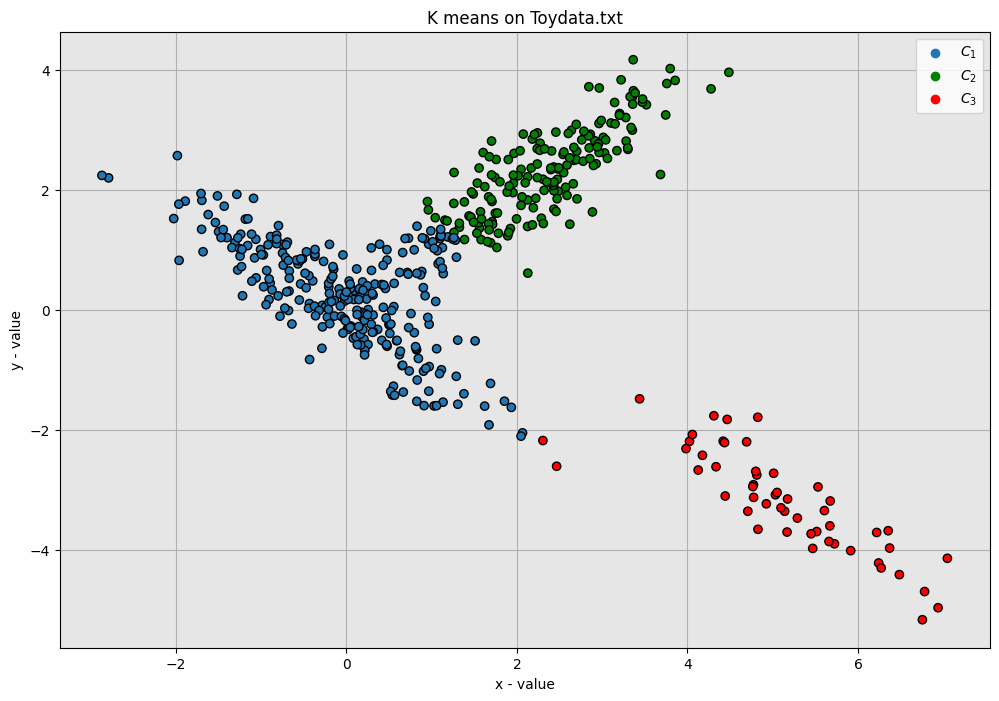
\includegraphics[width = 0.8\textwidth]{Figure/kmeans.png}
    \caption{$K$-means on Toy Data.}
    \label{fig:kmeans}
\end{figure}

\begin{figure}
    \centering
    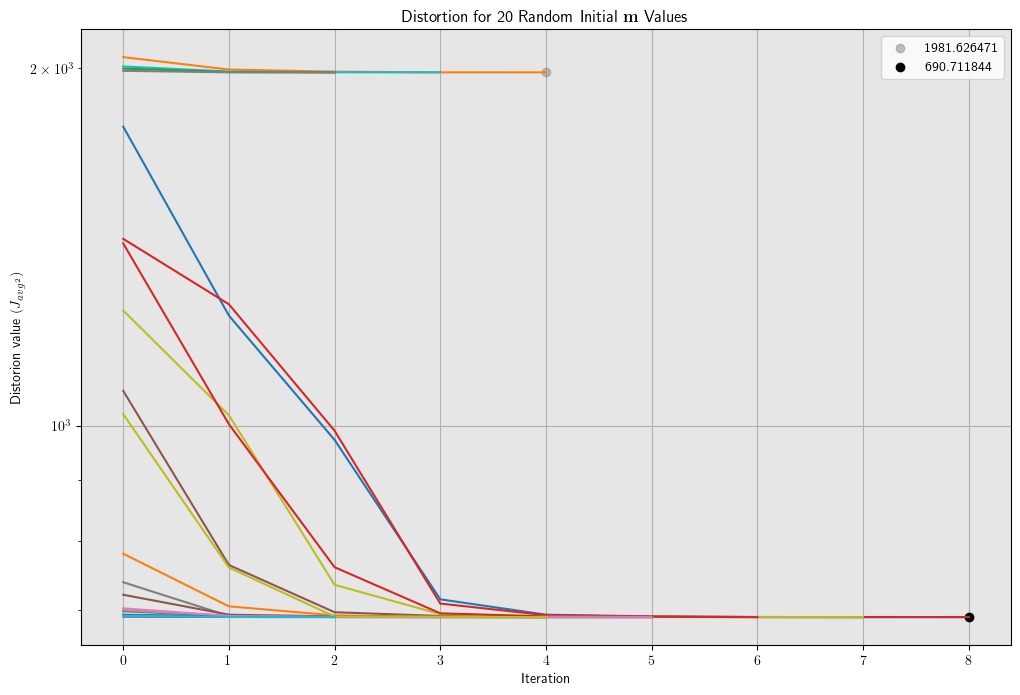
\includegraphics[width=0.8\textwidth]{Figure/Different vals.png}
    \caption{20 Different values and their converging minima.}
    \label{fig:Differentvals}
\end{figure}

\clearpage
\newpage
\subsection{Problem 2, part b}
Now implement the $k$–means++ algorithm discussed in class and repeat part (a) using its result as initialization (except for the 2D plot). Comment on the convergence behavior of $k$–means++ vs. the original algorithm.
\partbreak
\begin{solution}

    I have (hopefully) implemented the $k$-means++ algorithm correctly, and present the resulting distortion plot in Figure \ref{fig:k-means++}, we can see that the convergence for $k$-means++ is less (6 compared to 8), with one outlier condition, which ran for noticeably longer. All points converged to the global minimum, and the iterations needed to get to the minimum is 2 to 6 (with the outlier removed). 
\end{solution}

\vspace{4cm}
\begin{figure}[!ht]
    \centering
    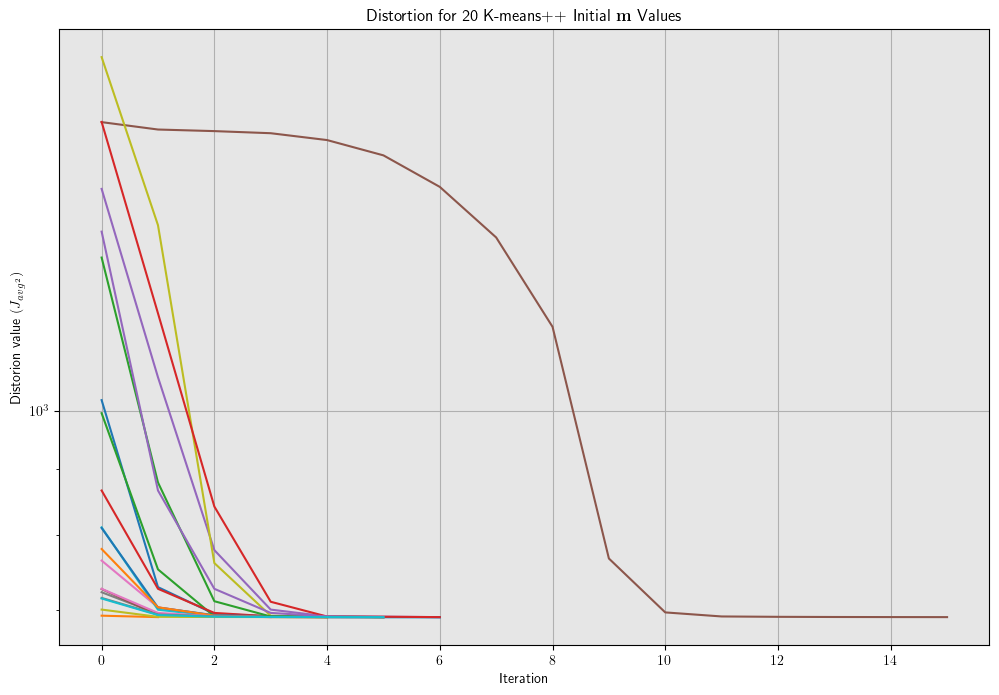
\includegraphics[width = 0.8\textwidth]{Figure/kmeans++.png}
    \caption{$k$-means initialized by $k$-means++.}
    \label{fig:k-means++}
\end{figure}

\clearpage
\newpage
\subsection{Problem 2, part c}
Test both the original k-means and k-means++ algorithms on the MNIST dataset. Each image in MNIST is 28x28 pixels, represented as a 784-dimensional vector. Again, comment on the convergence behavior of k-means++ vs. the original algorithm. Comment on how the results differ when you set the number of clusters to 10 and 16.
\partbreak
\begin{solution}

    The comparison plots are given below, with respect to all notable combinations. We see that $k$-means++ converges to the same minimum as $k$-means, but does it in consistently less iterations and lesser initial distortion value. For the difference in $k$-means++ and random initialization, we see an average iteration length of 86 and 100, respectively.  
\end{solution}

\newpage
\begin{figure}
    \centering
    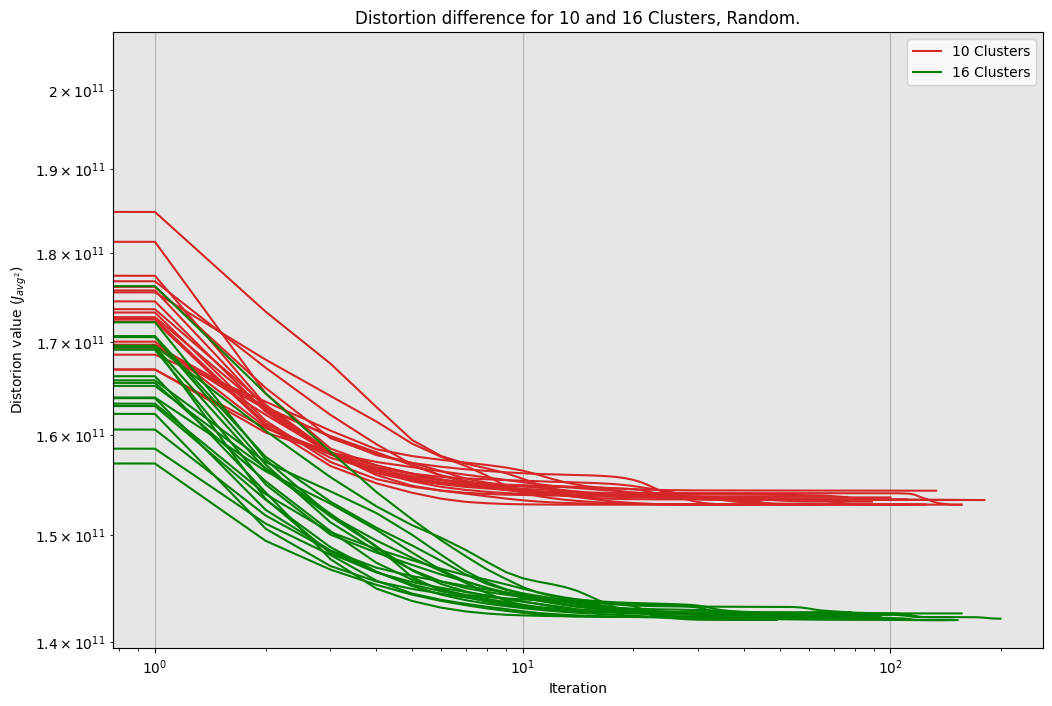
\includegraphics[width = 0.8\textwidth]{Figure/clusterdifferencerandom.png}
\end{figure}

\begin{figure}
    \centering
    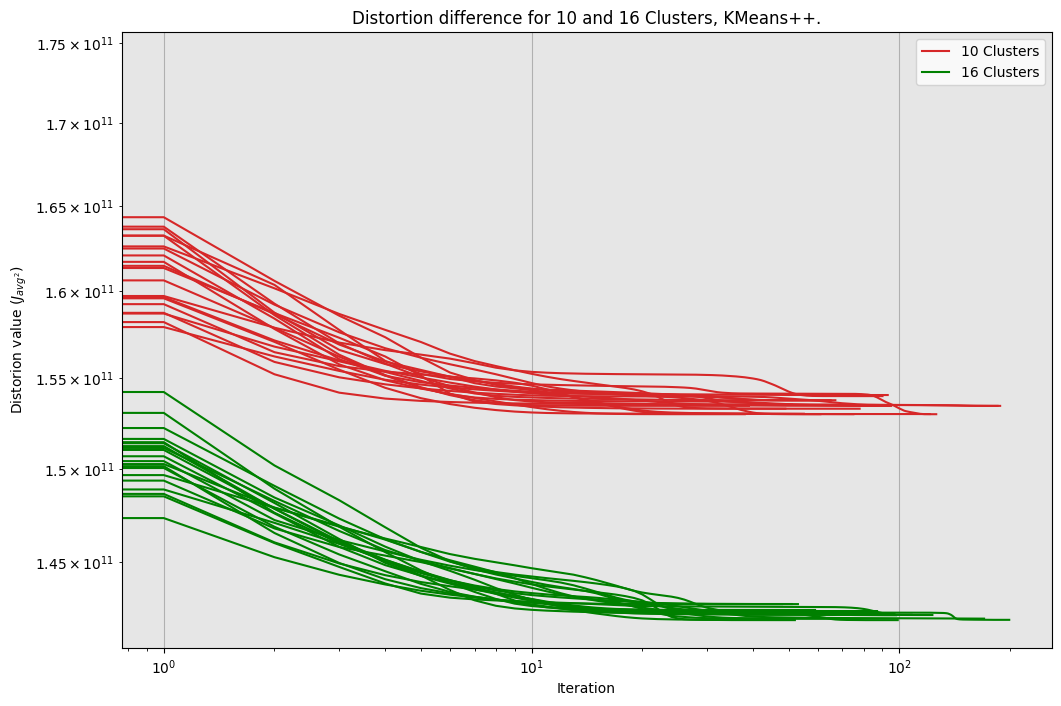
\includegraphics[width = 0.8\textwidth]{Figure/clusterdifferencekmeans.png}
\end{figure}


\begin{figure}
    \centering
    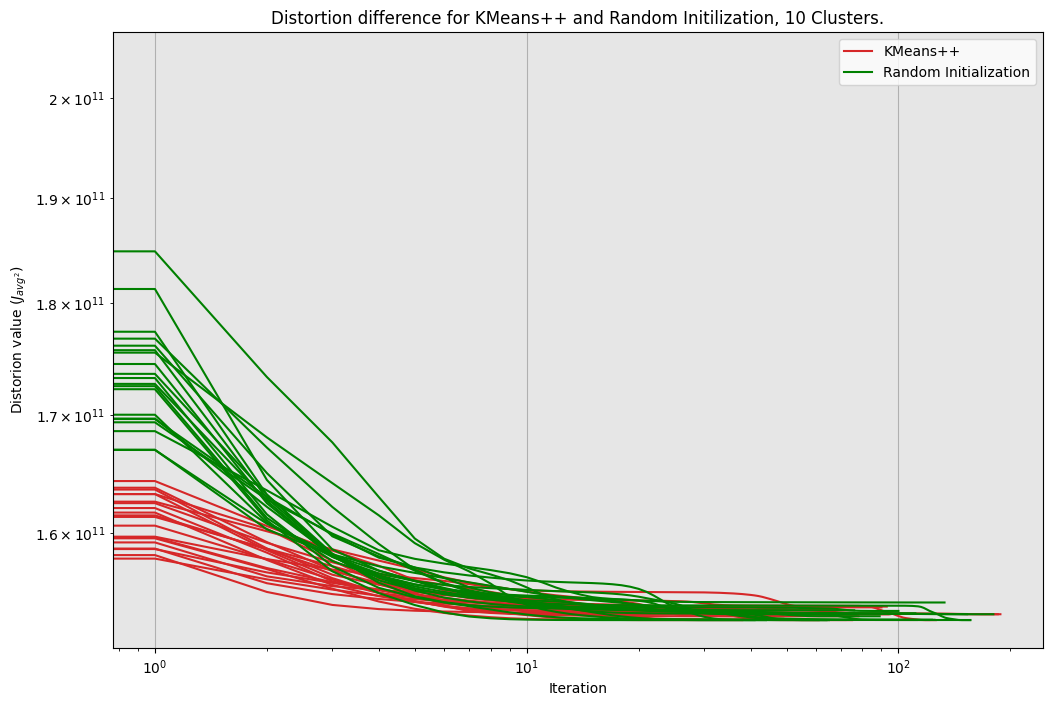
\includegraphics[width = 0.8\textwidth]{Figure/10clustersmnist.png}
\end{figure}

\begin{figure}
    \centering
    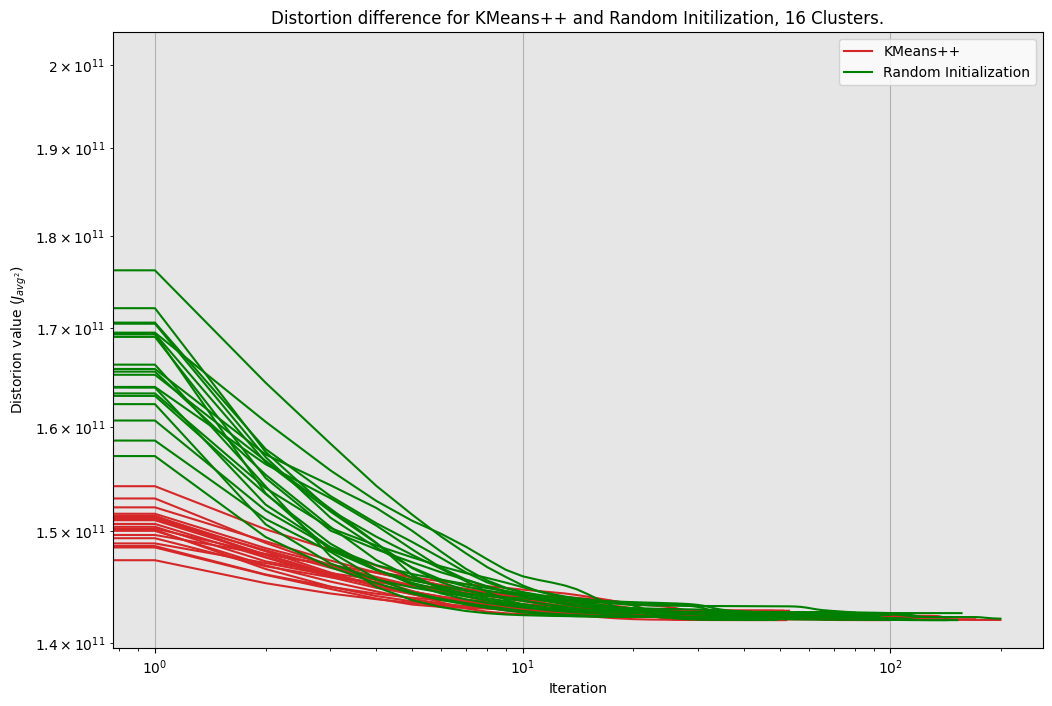
\includegraphics[width = 0.8\textwidth]{Figure/16clustersmnist.png}
\end{figure}

\clearpage


\newpage
\section{Problem 3}
Recall the "Mixture of $k$ Gaussians" model used in clustering
\begin{align}
    p(\textbf{x}, z) = \pi_z \scN (\textbf{x};\boldsymbol{\mu}_z, \boldsymbol{\Sigma}_z), \label{Gauss}
\end{align}
where $\textbf{x} \in \R^d, z \in \{1, 2, ..., k\}$ is its cluster assignment, and $\scN (\textbf{x};\boldsymbol{\mu}_z, \boldsymbol{\Sigma}_z)$ is the $d$-dimensional normal density
\[\scN (\textbf{x};\boldsymbol{\mu}_z, \boldsymbol{\Sigma}_z) = (2\pi)^{-d/2} |\boldsymbol{\Sigma}_z|^{-1/2} \exp \left( -(\textbf{x} - \boldsymbol{\mu}_z)\T \boldsymbol{\Sigma}_z\inv (\textbf{x} - \boldsymbol{\mu}_z) / 2\right).\]
The parameters of this restricted model are $\theta = (\pi_1, ..., \pi_k, \boldsymbol{\mu}_1, ..., \boldsymbol{\mu}_k, \boldsymbol{\Sigma}_1, ..., \boldsymbol{\Sigma}_k).$

\subsection{Problem 3, part a}
Let $\{(\textbf{x}_1, z_1), (\textbf{x}_2, z_2), ..., (\textbf{x}_n, z_n)\}$ be an $n$-point sample from this model. Write down the corresponding log-likelihood $\ell(\theta)$. As usual, you may ignore constant terms in the log-likelihood. 
\partbreak
\begin{solution}

    I am relatively new to statistics, so forgive me if my explanations are poorly written. The likelihood function seeks to describe a given set of parameters $\theta$ are more likely to be the true set of parameters, assuming we have fixed random variables $\textbf{x}$. Since the given parameters are discrete and constitute all probable cases for the model, we will sum over them for each random instance encountered. Furthermore, since each random instance is assumed independent, we have the likelihood function to be 
    \[L(\theta) = \prod_{i = 1}^n \sum_{j = 1}^k \pi_i \scN (\textbf{x}_j; \boldsymbol{\mu}_j, \boldsymbol{\Sigma}_j).\]
    This results in a log-likelihood function of 
    \[\ell(\theta) = \sum_{i =1}^n \ln\left(\sum_{j = 1}^k \pi_j \scN (\textbf{x}_i; \boldsymbol{\mu}_j, \boldsymbol{\Sigma}_j)\right)\]
    by properties of the natural log. I am refraining from expanding out the $\scN$ term, just to preserve ease of readability.
\end{solution}


\newpage
\subsection{Problem 3, part b}
Let $p_{i, j}$ be the probability $p(z_i = j | \textbf{x}_i)$ of the $i$-th data point coming from the $j$-th cluster (given that its position is $\textbf{x}_i$). Derive an expression for this probability.  
\partbreak
\begin{solution}

    Seeing as though this is an occurrence of one event happening from a set of $k$ events ($\textbf{x}_i$ being in the $j$-th cluster), we would imagine that the probability of this event occurring would result in the proportional behavior of the values of $j$ in the overall parameter $\theta$. In other words, we would set 
    \[p_{i, j} = \frac{p(\textbf{x}_i, j)}{\sum_{l = 1}^k p(\textbf{x}_i, l)} = \frac{\pi_j\scN(\textbf{x}; \boldsymbol{\mu}_j, \boldsymbol{\Sigma}_j)}{\sum_{l = 1}^k \pi_l \scN (\textbf{x}_i ; \boldsymbol{\mu}_l, \boldsymbol{\Sigma}_l)}.\]
\end{solution}

\newcommand{\lbarthetaold}{\overline{\ell}_{\theta_{old}}(\theta)}

\newpage
\subsection{Problem 3, part c}
Derive the expected log-likelihood $\lbarthetaold$ in terms of these $p_{i, j}$ conditional probabilities. Here the expectation is taken over the values of the hidden variables $(z_1, ..., z_n)$, and the subscript $\theta_{old}$ signifies that the $p_{i, j}'s$ are computed with respect to the old values of the parameters, whereas $\overline{\ell}$ itself is a function of the new values of the parameters. 
\partbreak
\begin{solution}

    The expected value of the log-likelihood is given as the general expected value formula, 
    \[E (\theta, \theta_{old}) = \sum_{l = 1}^k p_{i, l}\ln\left(p(\textbf{x}, z)\right),\]
    where the term in the natural log is the probability function of our new parameters, and $p_{i, l}$ is our old probabilities. This new probability represents the probability over all input data, $\textbf{x}$, thus, we can break them apart by data entry, to write
    \[E (\theta, \theta_{old}) = \sum_{l = 1}^k p_{i, l}\sum_{n = 1}^N\ln\left(\pi_n\scN(\textbf{x}_n; \boldsymbol{\mu}_n, \boldsymbol{\Sigma}_n)\right).\]
    Note that I have pulled out the product from the natural log and turned it into a sum. Since this new sum is independent of the old, we can pull it to the front as follows:
    \[E (\theta, \theta_{old}) = \sum_{n = 1}^N\sum_{l = 1}^k p_{i, l}\ln\left(\pi_n\scN(\textbf{x}_n; \boldsymbol{\mu}_n, \boldsymbol{\Sigma}_n)\right).\]
    Next, we notice the old conditional probability term is the expected value of the second term, implying that we can rewrite the expected value as
    \[E(\theta, \theta_{old}) =  \sum_{n = 1}^N\sum_{l = 1}^k p_{l, l}\ln\left(\pi_\scN(\textbf{x}_n; \boldsymbol{\mu}_n, \boldsymbol{\Sigma}_n)\right).\]

    Plugging in what we have, we see that the expectation value is of the form
    \[E(\theta, \theta_{old}) = \sum_{n = 1}^N\sum_{l = 1}^k p_{n, l} \left[ \ln(\pi_l) - \frac{d}{2}\ln (2\pi) - \frac{1}{2}\ln(|\det (\boldsymbol{\Sigma}_l)|) - \frac{1}{2}(\textbf{x}_n - \boldsymbol{\mu}_l)\T \boldsymbol{\Sigma}\inv_l (\textbf{x}_n - \boldsymbol{\mu}_l)\right]\]
\end{solution}

\newpage
\subsection{Problem 3, part d}
The expectation maximization algorithm updates the parameters of the mixture by maximizing $\lbarthetaold$. Let us start with the ``cluster priors'' $\pi_1, ..., \pi_k.$ Since $(\pi_1, ..., \pi_k)$ is a discrete distribution, we must have that $\sum_{j = 1}^k \pi_j = 1$. Using this constraint, derive the update rule for the cluster priors. 
\partbreak
\begin{solution}

    Taking the constraint we have on the cluster priors, we can substitute in a single term for the whole sum. In particular, when replacing the last cluster prior, we have that 
    \[\pi_k = 1 - \sum_{j = 1}^{k-1} \pi_j\]
    This will be used in differentiation. When finding the particular $pi_j$ which maximizes $\lbarthetaold$, we can employ simple calculus: taking the derivative with respect to $\pi_j$ and setting equal to zero. We see that, when differentiating, we should keep in mind the one instance of $p_{i, j}$ which is not a constant with respect to differentiation, in particular, $\pi_j$. Therefore, the sum over clusters can be dropped, since the only one which is not a constant is the $j$-cluster. We then see that, when differentiating, 
<<<<<<< HEAD:Quarter 3/Machine Learning/Homework/Homework1/main.tex
<<<<<<< HEAD
    \[\frac{d E}{d\pi_j} = \sum_{i = 1}^N \left[p_{i, j}\frac{1}{\pi_j} - p_{k, j}\frac{1}{1 - \sum_{l = 1}^{k-1} \pi_l}\right] = 0.\]
    After rearranging, we have that
    \[\frac{1}{\pi_j}\sum_i p_{i, j} = \frac{1}{1 - \sum_{j = 1}^{k-1} \pi_j}\sum_i p_{k, j}. \]
    Finally, after simplification, we have
    \[\pi_j = \frac{1}{N}\sum_{i = 1}^N p_{i, j}.\]
    
\end{solution}


\newpage
\subsection{Problem 3, part e}
Similarly derive the update rule for the $\boldsymbol{\mu}_1, ..., \boldsymbol{\mu}_k$ location parameters and $\boldsymbol{\Sigma}_1, ..., \boldsymbol{\Sigma}_k$ covariance matrices. 
\vspace{-2mm}\partbreak\vspace{-2mm}
\begin{solution}

    The update rules for $\boldsymbol{\mu}$ and $\boldsymbol{\Sigma}$ are done similarly. We will show the update scheme for the $\boldsymbol{\mu}$'s first, then the $\boldsymbol{\Sigma}$'s after. 
    \tightalignbreak\vspace{-2mm}
    \begin{align*}
        &\grad_{\boldsymbol{\mu}_j} = E(\theta, \theta_{old}) &\text{(Given.)}\\
        &= -\frac{1}{2}\sum_{i = 1}^N p_{i, j} \grad_{\boldsymbol{\mu}_j}(\textbf{x}_i - \boldsymbol{\mu}_j) \boldsymbol{\Sigma}\inv_j (\textbf{x}_i - \boldsymbol{\mu}_j) &\text{(Simplifying.)}\\
        &= -\frac{1}{2}\sum_{i = 1}^N p_{i, j} (2\boldsymbol{\Sigma}\inv_j \textbf{x}_i + 2\boldsymbol{\Sigma}\inv_j \boldsymbol{\mu}_j) = 0 &\text{(Simplifying and setting to zero.)}\\
        \implies & \boldsymbol{\Sigma}\inv_j\boldsymbol{\mu}_j\sum_{i = 1}^Np_{i, j} = \sum_{i = 1}^N p_{i, j}\boldsymbol{\Sigma}\inv_j \textbf{x}_i &\text{(Rearranging.)}\\
        \boldsymbol{\mu}_j &= \frac{\sum_{i = 1}^N{p_{i, j}\textbf{x}_i}}{\sum_{i = 1}^N{p_{i, j}}} &\text{(Simplifying.)}
    \end{align*}
    \vspace{-12mm}\alignbreak\vspace{-6mm}
    \begin{align*}
        &\grad_{\boldsymbol{\Sigma}\inv_j} E(\theta, \theta_{old}) = \sum_{i = 1}^N p_{i, j} \grad \left[ -\frac{1}{2} \ln{(|\det \boldsymbol{\Sigma}_j)|}  - \frac{1}{2}(\textbf{x}_i - \boldsymbol{\mu}_j)\T \boldsymbol{\Sigma}\inv_j (\textbf{x}_i - \boldsymbol{\mu}_j)\right] &\text{(Applying Gradient.)}\\
        &= \sum_{i = 1}^N p_{i, j} \grad \left[ \frac{1}{2} \ln{(|\det \boldsymbol{\Sigma}\inv_j|)}  - \frac{1}{2}(\textbf{x}_i - \boldsymbol{\mu}_j)\T \boldsymbol{\Sigma}\inv_j (\textbf{x}_i - \boldsymbol{\mu}_j)\right] &\text{(inverse properties.)}\\
        &= \sum_{i = 1}^N p_{i, j} \left[ ((\boldsymbol{\Sigma}\inv_j)\T)\inv - \frac{1}{2}(\textbf{x}_i - \boldsymbol{\mu}_j)\T \boldsymbol{\Sigma}\inv_j (\textbf{x}_i - \boldsymbol{\mu}_j)\right] &(\bigstar)\\
        &= \sum_{i = 1}^N p_{i, j} \left[ ((\boldsymbol{\Sigma}\inv_j)\T)\inv - (\textbf{x}_i - \boldsymbol{\mu}_j) (\textbf{x}_i - \boldsymbol{\mu}_j)\T \right] &(\bigstar \bigstar)\\
        &= \sum_{i = 1}^N p_{i, j} \left[ \boldsymbol{\Sigma}_j - (\textbf{x}_i - \boldsymbol{\mu}_j) (\textbf{x}_i - \boldsymbol{\mu}_j)\T \right] &\text{($\boldsymbol{\Sigma}_j$ is symmetric.)}\\
        &\implies \boldsymbol{\Sigma}_j \sum_{i = 1}^N p_{i, j} = \sum_{i = 1}^N p_{i, j}(\textbf{x}_i - \boldsymbol{\mu}_j)(\textbf{x}_i - \boldsymbol{\mu}_j)\T  &\text{(Setting to zero.)}\\
        &\boldsymbol{\Sigma}_j = \frac{\sum_{i = 1}^N p_{i, j}(\textbf{x}_i - \boldsymbol{\mu}_j)(\textbf{x}_i - \boldsymbol{\mu}_j)\T}{\sum_{i = 1}^N p_{i, j}}
    \end{align*}
    \vspace{-12mm} \alignbreak

    The lines labelled ($\bigstar$) and ($\bigstar \bigstar$) come from The Matrix Cookbook, https://www.math.uwaterloo.ca/~hwolkowi/matrixcookbook.pdf, equations 57 and 72, respectively.  
\end{solution}

\newpage
\subsection{Problem 3, part f}
Compare these update rules to the $k$-means update rules derived in Question 1. 
\partbreak
\begin{solution}

    the only update scheme we found in Problem 1 was the centroid update within a given cluster. This formula resembles the cluster priors, with a notable difference that we are summing over all data points, rather than the cluster paradigm seen in $k$-means.   
\end{solution}

\newpage
\subsection{Problem 3, part g}
Apply the Mixture of Gaussians clustering algorithm to the toy data in Question 2. Plot the final result as a 2D plot in which each point's color or symbol indicates its cluster assignment. Comment on the plot and the convergence speed compared to that of $k$-means. 

=======
    \[\frac{d E}{d\pi_j} = \sum_{i = 1}^N \left[p_{i, j}\frac{1}{\pi_j} - p_{k, j}\frac{1}{1 - \sum_{l = 1}^{k-1} \pi_l}\right] = 0\]
=======
    \[\frac{d E}{d\pi_j} = \sum_{i = 1}^N \left[p_{i, j}\frac{1}{\pi_j} - p_{k, j}\frac{1}{1 - \sum_{l = 1}^{k-1} \pi_l}\right] = 0.\]
>>>>>>> d022d703bbd96ccdcbfc60ce38fd00b823f2cd5d:main.tex
    After rearranging, we have that
    \[\frac{1}{\pi_j}\sum_i p_{i, j} = \frac{1}{1 - \sum_{j = 1}^{k-1} \pi_j}\sum_i p_{k, j}. \]
    Finally, after simplification, we have
    \[\pi_j = \frac{1}{N}\sum_{i = 1}^N p_{i, j}.\]
    
\end{solution}
<<<<<<< HEAD:Quarter 3/Machine Learning/Homework/Homework1/main.tex
>>>>>>> 3bfa73585ae21296371bbef57ed1d1adc1a50a69
=======


\newpage
\subsection{Problem 3, part e}
Similarly derive the update rule for the $\boldsymbol{\mu}_1, ..., \boldsymbol{\mu}_k$ location parameters and $\boldsymbol{\Sigma}_1, ..., \boldsymbol{\Sigma}_k$ covariance matrices. 
\vspace{-2mm}\partbreak\vspace{-2mm}
\begin{solution}

    The update rules for $\boldsymbol{\mu}$ and $\boldsymbol{\Sigma}$ are done similarly. We will show the update scheme for the $\boldsymbol{\mu}$'s first, then the $\boldsymbol{\Sigma}$'s after. 
    \tightalignbreak\vspace{-2mm}
    \begin{align*}
        &\grad_{\boldsymbol{\mu}_j} = E(\theta, \theta_{old}) &\text{(Given.)}\\
        &= -\frac{1}{2}\sum_{i = 1}^N p_{i, j} \grad_{\boldsymbol{\mu}_j}(\textbf{x}_i - \boldsymbol{\mu}_j) \boldsymbol{\Sigma}\inv_j (\textbf{x}_i - \boldsymbol{\mu}_j) &\text{(Simplifying.)}\\
        &= -\frac{1}{2}\sum_{i = 1}^N p_{i, j} (2\boldsymbol{\Sigma}\inv_j \textbf{x}_i + 2\boldsymbol{\Sigma}\inv_j \boldsymbol{\mu}_j) = 0 &\text{(Simplifying and setting to zero.)}\\
        \implies & \boldsymbol{\Sigma}\inv_j\boldsymbol{\mu}_j\sum_{i = 1}^Np_{i, j} = \sum_{i = 1}^N p_{i, j}\boldsymbol{\Sigma}\inv_j \textbf{x}_i &\text{(Rearranging.)}\\
        \boldsymbol{\mu}_j &= \frac{\sum_{i = 1}^N{p_{i, j}\textbf{x}_i}}{\sum_{i = 1}^N{p_{i, j}}} &\text{(Simplifying.)}
    \end{align*}
    \vspace{-12mm}\alignbreak\vspace{-6mm}
    \begin{align*}
        &\grad_{\boldsymbol{\Sigma}\inv_j} E(\theta, \theta_{old}) = \sum_{i = 1}^N p_{i, j} \grad \left[ -\frac{1}{2} \ln{(|\det \boldsymbol{\Sigma}_j)|}  - \frac{1}{2}(\textbf{x}_i - \boldsymbol{\mu}_j)\T \boldsymbol{\Sigma}\inv_j (\textbf{x}_i - \boldsymbol{\mu}_j)\right] &\text{(Applying Gradient.)}\\
        &= \sum_{i = 1}^N p_{i, j} \grad \left[ \frac{1}{2} \ln{(|\det \boldsymbol{\Sigma}\inv_j|)}  - \frac{1}{2}(\textbf{x}_i - \boldsymbol{\mu}_j)\T \boldsymbol{\Sigma}\inv_j (\textbf{x}_i - \boldsymbol{\mu}_j)\right] &\text{(inverse properties.)}\\
        &= \sum_{i = 1}^N p_{i, j} \left[ ((\boldsymbol{\Sigma}\inv_j)\T)\inv - \frac{1}{2}(\textbf{x}_i - \boldsymbol{\mu}_j)\T \boldsymbol{\Sigma}\inv_j (\textbf{x}_i - \boldsymbol{\mu}_j)\right] &(\bigstar)\\
        &= \sum_{i = 1}^N p_{i, j} \left[ ((\boldsymbol{\Sigma}\inv_j)\T)\inv - (\textbf{x}_i - \boldsymbol{\mu}_j) (\textbf{x}_i - \boldsymbol{\mu}_j)\T \right] &(\bigstar \bigstar)\\
        &= \sum_{i = 1}^N p_{i, j} \left[ \boldsymbol{\Sigma}_j - (\textbf{x}_i - \boldsymbol{\mu}_j) (\textbf{x}_i - \boldsymbol{\mu}_j)\T \right] &\text{($\boldsymbol{\Sigma}_j$ is symmetric.)}\\
        &\implies \boldsymbol{\Sigma}_j \sum_{i = 1}^N p_{i, j} = \sum_{i = 1}^N p_{i, j}(\textbf{x}_i - \boldsymbol{\mu}_j)(\textbf{x}_i - \boldsymbol{\mu}_j)\T  &\text{(Setting to zero.)}\\
        &\boldsymbol{\Sigma}_j = \frac{\sum_{i = 1}^N p_{i, j}(\textbf{x}_i - \boldsymbol{\mu}_j)(\textbf{x}_i - \boldsymbol{\mu}_j)\T}{\sum_{i = 1}^N p_{i, j}}
    \end{align*}
    \vspace{-12mm} \alignbreak

    The lines labelled ($\bigstar$) and ($\bigstar \bigstar$) come from The Matrix Cookbook, https://www.math.uwaterloo.ca/~hwolkowi/matrixcookbook.pdf, equations 57 and 72, respectively.  
\end{solution}

\newpage
\subsection{Problem 3, part f}
Compare these update rules to the $k$-means update rules derived in Question 1. 
\partbreak
\begin{solution}

    The only update scheme we found in Problem 1 was the centroid update within a given cluster. This formula resembles the cluster priors, with a notable difference that we are summing over all data points, rather than the cluster paradigm seen in $k$-means.   
\end{solution}

\newpage
\subsection{Problem 3, part g}
Apply the Mixture of Gaussians clustering algorithm to the toy data in Question 2. Plot the final result as a 2D plot in which each point's color or symbol indicates its cluster assignment. Comment on the plot and the convergence speed compared to that of $k$-means. 
\partbreak

\begin{solution}

    I have spent a significant amount of time typing this from scratch in C++ and debugging the whole thing. My best results are shown below. I am not aware of the exact value we should be seeing for the log likelihood, but the results incorrectly cluster all points into the third cluster. This could result from my incorrect initialization of the covariance matrices, since my initial values are just random points within our space. I will include all my code in submission, just for confirmation. 
\end{solution}

\newpage
\begin{figure}
    \centering
    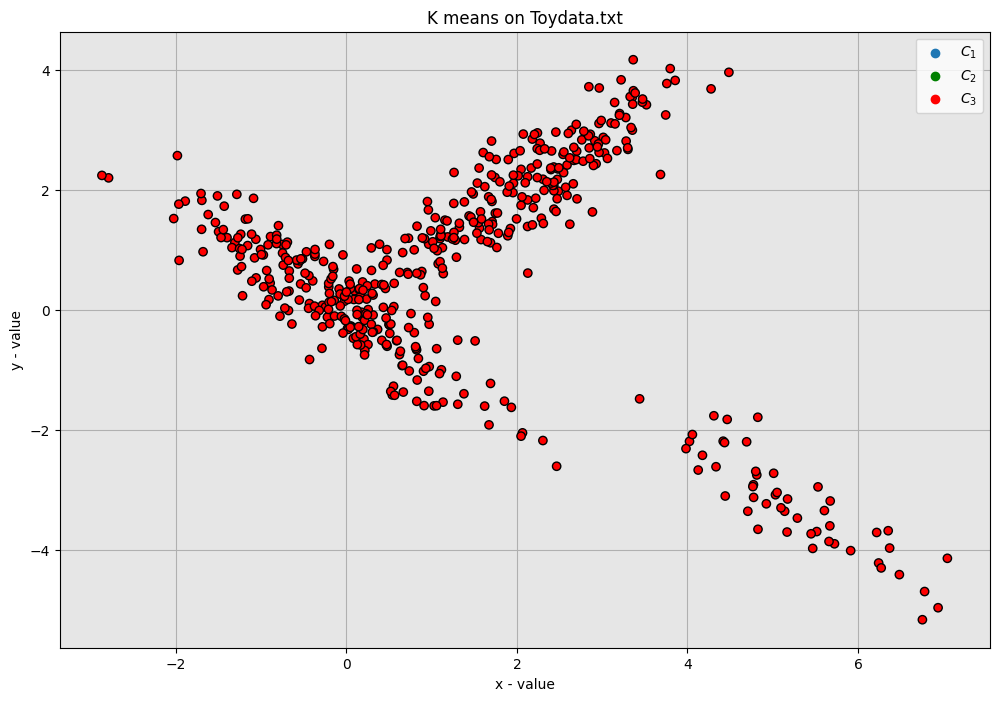
\includegraphics[width = 0.8\textwidth]{Figure/gaussiancluster.png}
\end{figure}

\begin{figure}
    \centering
    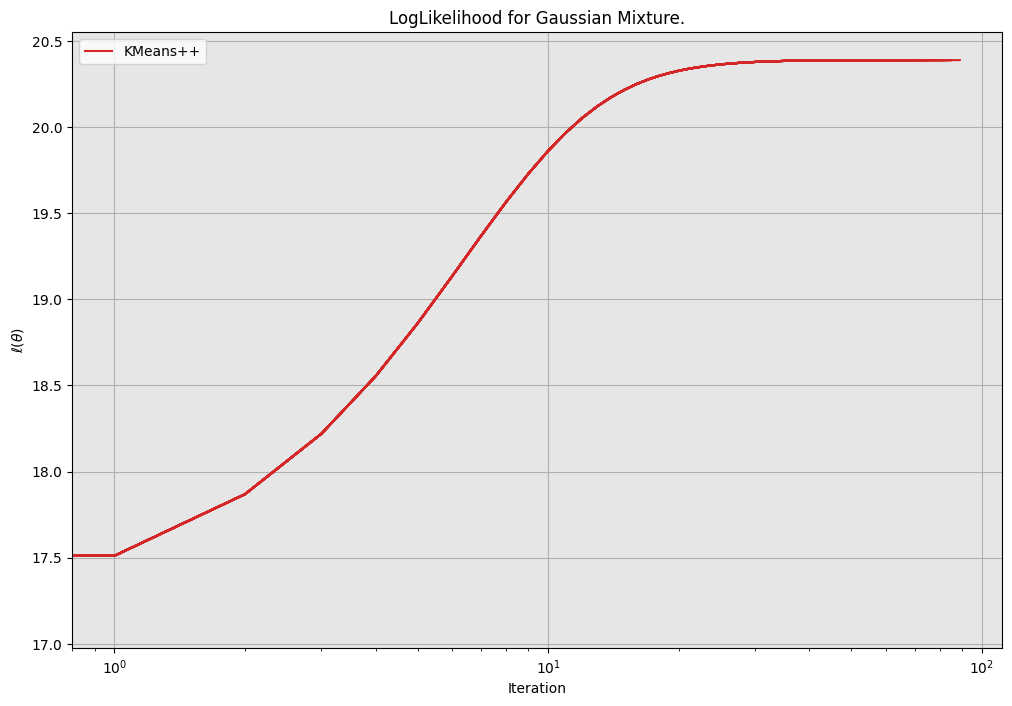
\includegraphics[width = 0.8\textwidth]{Figure/loglikelihood.png}
\end{figure}

\clearpage
\newpage

\section{Problem 4}
You likely found that on the “toydata” dataset, most of the time even vanilla k–means clustering produces acceptable solutions. Create a dataset of your own for which (on average over many runs) k–means++ improves the performance of k–means by at least a factor of 10 in terms of the distortion function value of the final clustering. Submit the code that you used to generate the dataset.

\partbreak
\begin{solution}

    A "nice" example of a dataset which would generate this disparity is for there to be two clusters of data points, far from each other, where we initialize $k = 2$. This can be done for arbitrary number of clusters, we just require there to be an equal number of clusters of data sufficiently far from each other. In this example, $k$-means++ will always initialize (or be heavily weighted toward) choosing the initial cluster centroids within different clusters of data, whereas random initialization will have a chance of selecting points within the same cluster as initial steps. Since the two clusters are sufficiently far apart, a cluster centroid will never average out into the other cluster, which would significantly decrease the distortion function. Therefore, we can see that for sufficient distance, we will attain an average distortion function ratio of 10. An example of this is given for the following points in 2D space: 
\begin{lstlisting}
-10.0, 1.0
-10.0, -1.0
10.0, 1.0
10.0, -1.0
\end{lstlisting}

Note the two clusters appearing at -10 and 10 on the x axis. More data points can be included, but this is a concise example to illustrate the disparity.  

\end{solution}


>>>>>>> d022d703bbd96ccdcbfc60ce38fd00b823f2cd5d:main.tex
\end{document}